\documentclass{article}
\usepackage[utf8]{inputenc}
\usepackage[margin=1.0in]{geometry}
\usepackage{amsmath,amsfonts,amssymb,amsthm}
\usepackage{enumerate}
\usepackage{dsfont}
\usepackage{physics}
\usepackage{tensor}
\usepackage{siunitx}
\usepackage{mathtools}
\usepackage{cancel}
%\usepackage{graphicx}
\usepackage{bigints}
\usepackage{tikz}
%\usepackage{hyperref}

\newcommand{\iu}{{i\mkern1mu}}

\title{Proyecto 1.}
\author{Cristian David Gutiérrez}
\date{}

\begin{document}

\maketitle

\section{Ecuación de Schrödinger en una dimensión.}

La evolución temporal de un ket de estado $\ket{\psi(x)}$ está gobernado por la ecuación de Schrödinger en una dimensión:

\begin{equation*}
    \iu\hbar\dv{t}\ket{\psi(x)}=\hat{H}(t)\ket{\psi(x)}
\end{equation*}

Donde $\hat{H}(t)$ es un operador asociado al observable de energía del sistema, llamado hamiltoniano. Clásicamente, el hamiltoniano de una partícula de masa $m$, con momentum lineal $p$ y sujeta a un potencial $V$ escalar que únicamente depende de la posición $x$ de la partícula, es:

\begin{equation*}
    \mathcal{H}=\frac{p^2}{2m}+V(x)
\end{equation*}


Puede mostrarse que para la descripción cuántica basta con promover las cantidades $p$ y $x$ a operadores $\hat{p}$ y $\hat{x}$, y por tanto el hamiltoniano está dado por

\begin{equation*}
    \hat{H}=\frac{\hat{p}^2}{2m}+V(\hat{x})
\end{equation*}

Si escogemos la representación de posición donde el estado es representado mediante la función de onda $\Psi(x,t)$,  $\hat{p}=\iu\hbar\pdv*{x}$ y $\hat{x}=x$, la ecuación de Schrödinger es

\begin{equation}
    \iu\hbar\pdv{t}\Psi(x,t)=-\frac{\hbar^2}{2m}\pdv[2]{x}\Psi(x,t)+V(x)\Psi(x,t)
\end{equation}

Una forma de resolver esta ecuación diferencial es mediante el método de separación de variables, si la función $\Psi(x,t)$ se puede separar como un producto de la forma $\Psi(x,t)=\psi(x)\phi(t)$, la ecuación anterior queda de la siguiente forma

\begin{equation*}
\begin{split}
    \iu\hbar\psi(x)\dv{t}\phi(t)&=\phi(t)\qty[-\frac{\hbar^2}{2m}\dv[2]{x}\psi(x)+V(x)\psi(x)]\\
    \frac{\iu\hbar}{\phi(t)}\dv{t}\phi(t)&=\frac{1}{\psi(x)}\qty[-\frac{\hbar^2}{2m}\dv[2]{x}\psi(x)+V(x)\psi(x)]\\
    F(t)&=G(x)
\end{split}
\end{equation*}

Se ha llegado a una igualdad entre dos funciones de variables diferentes e independientes, lo que es verdad siempre que $F(t)=E=G(x)$, con $E$ una constante; de manera que la ecuación se ha separado en dos:

\begin{equation}
    G(x)=E \longrightarrow -\frac{\hbar^2}{2m}\dv[2]{x}\psi(x)+V(x)\psi(x)=E\psi(x)
\end{equation}
\begin{equation}
    F(t)=E \longrightarrow \dv{t}\phi(t)=-\frac{\iu E}{\hbar}\phi(t)
\end{equation}

La ecuación (2) se puede resumir en la expresión $H(p,x)\psi(x)=E\psi(x)$, conocido como el problema de autovalores del operador diferencial $H(p,x)$, en el que las soluciones o autofunciones son indexadas por el autovalor $E=E_n$, tal que $H(p,x)\psi_n(x)=E_n\psi_n(x)$. Lo que hace que la solución a la ecuación (3) sean de la forma $\phi_n(t)=\exp{-\frac{\iu E_n}{\hbar}t}$, que debido al caracter lineal de la ecuación original, hace que la solución general sea

\begin{equation}
    \Psi(x,t)=\sum_{n=0}^{\infty}c_n\phi_n(t)\psi_n(x)=\sum_{n=0}^{\infty}c_n\exp{-\frac{\iu}{\hbar}E_n t}\psi_n(x)
\end{equation}

Bajo la condición de normalización $\int\dd{x}\Psi^{*}(x,t)\Psi(x,t)$=1 se sigue que los coeficientes son tales que

\begin{equation*}
    \sum_{n}|c_n|^2=1
\end{equation*}

Si en particular se restringen a valores reales:

\begin{equation}
    \sum_{n}c_n^2=1
\end{equation}

\section{Algoritmo para la solución.}

A continuación se desarrolla un algoritmo para hallar las autofunciones en el problema de autovalores antes presentado:

\begin{equation*}
    \qty[-\frac{\hbar^2}{2m}\dv[2]{x}+V(x)]\psi(x)=E_n\psi(x)
\end{equation*}

Si el potencial es una constante , $V_0$, fuera de la región $-a/2\leq x\leq a/2$; al multiplicar por $m/\hbar^2$ y haciendo adimensional el argumento de las funciones:

\begin{equation}
    \qty[-\frac{1}{2}\dv[2]{\eta}+\frac{m a^2}{\hbar^2}V(\eta)]\psi(\eta)=\frac{E m a^2}{\hbar^2}\psi(\eta), \qquad \eta\equiv \frac{x}{a}
\end{equation}

El algoritmo se trata de convertir este problema de autovalores para un operador diferencial en un problema de autovalores matricial; para ello recurrimos al método de diferencias finitas, la variable $\eta$ está definida en $-1\leq \eta\leq1$ y definimos $\Delta\eta=2/N$, de manera que el intervalo se ha discretizado en $N$ puntos $\eta_j$. Con esto se hacen las siguientes conversiones:

\begin{equation}
\begin{split}
    \psi(\eta)&\longrightarrow\psi(\eta_j)\equiv\psi_j\\
    V(\eta)&\longrightarrow V(\eta_j)\equiv V_j\\
    \dv[2]{\psi(\eta)}{\eta}&\longrightarrow \frac{\psi(\eta_{j+1})-2\psi(\eta_j)+\psi(\eta_{j-1})}{\Delta \eta^2}\equiv\frac{\psi_{j+1}-2\psi_j+\psi_{j-1}}{\Delta \eta^2}
\end{split}
\end{equation}

Reemplazando en (5)

\begin{equation*}
    -\frac{1}{2\Delta \eta^2}\psi_{j+1}+\qty[\frac{1}{\Delta\eta^2}+\frac{m a^2}{\hbar^2}V_j]\psi_j-\frac{1}{2\Delta\eta^2}\psi_{j-1}=\frac{E m a^2}{\hbar^2}\psi_j
\end{equation*}

Esta expresión se puede escribir en forma matricial

\begin{equation}
    \mqty(\frac{1}{\Delta\eta^2}+\frac{m a^2}{\hbar^2}V_1 & -\frac{1}{2\Delta\eta^2} & 0 & \dots & 0\\
    -\frac{1}{2\Delta\eta^2} & \frac{1}{\Delta\eta^2}+\frac{m a^2}{\hbar^2}V_2 & -\frac{1}{2\Delta\eta^2} & \dots & 0\\
    \vdots & \vdots & \vdots & \ddots & \vdots\\
    0 & 0 & 0 & -\frac{1}{2\Delta\eta^2} & \frac{1}{\Delta\eta^2}+\frac{m a^2}{\hbar^2}V_{N-1})\mqty(\psi_1\\ \psi_2\\ \vdots \\ \psi_{N-1})=\frac{E m a^2}{\hbar^2}\mqty(\psi_1\\ \psi_2\\ \vdots \\ \psi_{N-1})
\end{equation}

Un problema de autovalores de la forma $A\va{X}=\lambda\va{X}$ que es fácilmente soluble computacionalmente. Hay que agregar las condiciones sobre la frontera del intervalo, $\psi_0=A_0$ y $\psi_N=A_N$, siendo estas constantes $A_0, A_N$ determinadas a través de las soluciones fuera del potencial, donde es una constante.

\subsection{Soluciones fuera del potencial.}

Si fuera del intervalo $[-1,1]$ el potencial es constate e igual a $V_0$, entonces la ecuación de Schrödinger adimensional es

\begin{equation*}
    \dv[2]{\psi(\eta)}{\eta}+\frac{2 m a^2}{\hbar^2}(E-V_0)\psi(\eta)=0
\end{equation*}

Cuya solución es

\begin{equation}
    \psi(\eta)=A\exp{-\frac{2ma^2}{\hbar^2}(E-V_0)\abs{\eta}} \qquad \abs{\eta}>1
\end{equation}

Con las condiciones de frontera

\begin{equation*}
    \psi(\eta_0)=\psi_0=A\exp{-\frac{2ma^2}{\hbar^2}(E-V_0)}=\psi_N=\psi(\eta_N)
\end{equation*}

\section{Soluciones halladas.}

\subsection{Pozo Finito.}

Según el potencial entregado, las autofunciones y los autovalores devueltos por el algoritmo son

\begin{figure}[htp]
    \centering
    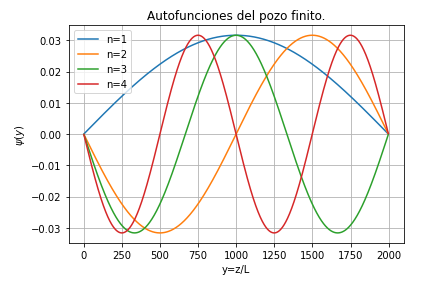
\includegraphics[scale=0.5]{finw_eigf.png}
    \caption{Autofunciones del pozo finito en la variable adimensional $y=x/L$}
    \label{fig:my_label}
\end{figure}

\begin{figure}[htp]
    \centering
    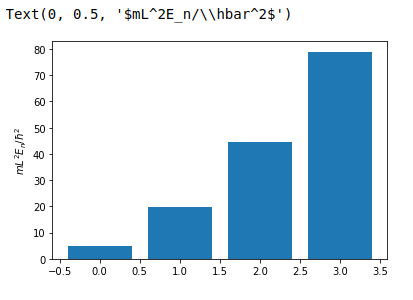
\includegraphics[scale=0.5]{finw_eigv.png}
    \caption{Autovalores del pozo finito en unidades $mL^2E_n/\hbar^2$}
    \label{fig:my_label}
\end{figure}

Se sabe que la densidad de probabilidad es proporcional al módulo cuadrado de la función de onda $|\psi_n(y)|^2$, la gráfica a continuación presenta esta densidad de probabilidad.

\begin{figure}[htp]
    \centering
    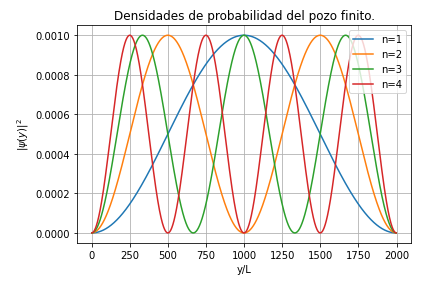
\includegraphics[scale=0.5]{finw_dens.png}
    \caption{Densidades de probabilidad para el pozo de potencial finito.}
    \label{fig:my_label}
\end{figure}

%\newpage
La solución dependiente del tiempo se construye a partir de los autoestados del hamiltoniano $\psi_{n}(y)$, como la combinación 

\begin{equation}
    \Psi(y,t)=\sum_{n=1}^{4}c_n\mathrm{e}^{-\iu E_n t/\hbar}\psi_n(y)
\end{equation}

Donde los coeficientes $c_n$ se escogen según la normalización (5) y aleatoriamente.

\begin{figure}[htp]
    \centering
    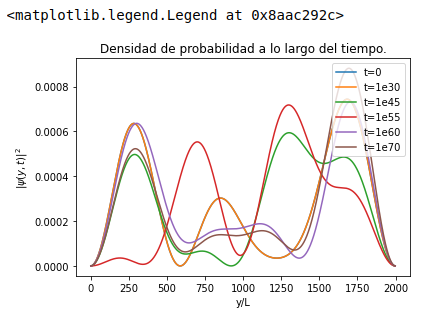
\includegraphics[scale=0.5]{finw_dens_t.png}
    \caption{Densidades de probabilidad para el pozo de potencial finito.}
    \label{fig:my_label}
\end{figure}

Por las condiciones sobre los parámetros como la masa y la constante de Planck reducida $\hbar$, las escalas de tiempo deben ser muy grandes para notar cambios en la densidad de probabilidad.



\subsection{Pozo Infinito.}

Haciendo que la altura del pozo finito sea mucho mayor que su ancho $h\gg l$, se puede obtener una aproximación para el pozo infinito, a continuación se muestran sus autofunciones

\begin{figure}[htp]
    \centering
    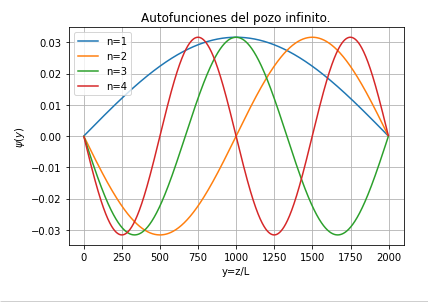
\includegraphics[scale=0.5]{infw_eigf.png}
    \caption{Autofunciones del pozo infinito en la variable adimensional $y=x/L$}
    \label{fig:my_label}
\end{figure}

\newpage
Y los autovalores respectivos.

\begin{figure}[htp]
    \centering
    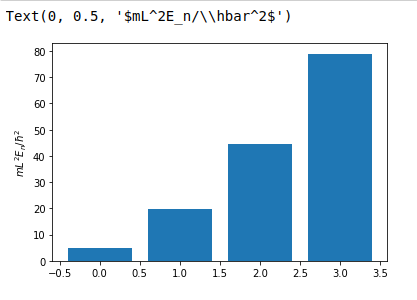
\includegraphics[scale=0.5]{infw_eigv.png}
    \caption{Autovalores del pozo infinito en unidades $mL^2E_n/\hbar^2$}
    \label{fig:my_label}
\end{figure}

\newpage
Además de las densidades de probabilidad.

\begin{figure}[htp]
    \centering
    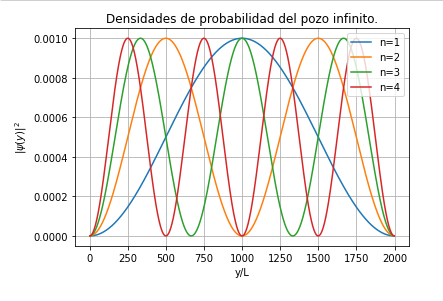
\includegraphics[scale=0.5]{infw_dens.png}
    \caption{Densidades de probabilidad para el pozo de potencial infinito.}
    \label{fig:my_label}
\end{figure}

Al igual que para el potencial finito, los coeficientes para la solución dependiente del tiempo se escogieron aleatoriamente y satisfaciendo la condición de normalización (5).

\begin{figure}[htp]
    \centering
    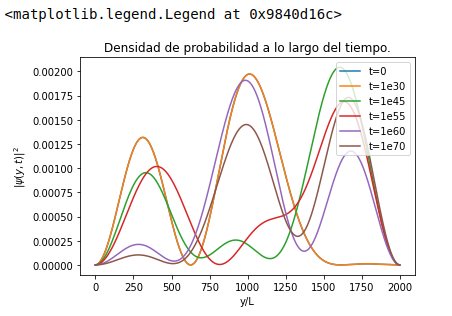
\includegraphics[scale=0.5]{infw_dens_t.png}
    \caption{Autovalores del pozo infinito en unidades $mL^2E_n/\hbar^2$}
    \label{fig:my_label}
\end{figure}


Debido a que el potencial para ambos pozos vale $0$ dentro de las paredes, las autofunciones y los autovalores son iguales; debido a la forma en que se programó el algoritmo, las condiciones iniciales para cada potencial son fijas $\psi(-a/2)=\psi(a/2)=0$, lo que da lugar a la igualdad de las autofunciones y autovalores. Además, el algoritmo no puede distinguir entre autofunciones acotadas y por ello los autovalores para el pozo finito pueden corresponder a funciones no ligadas. Es por esto que el algoritmo programado no puede resolver el problema del pozo finito.

%\newpage
\subsection{Potencial Cuadrático.}

Cambiando el potencial a la forma $V(y)=y^2$, las autofunciones del potencial halladas se muestran en la figura

\newpage
\begin{figure}[h]
\centering
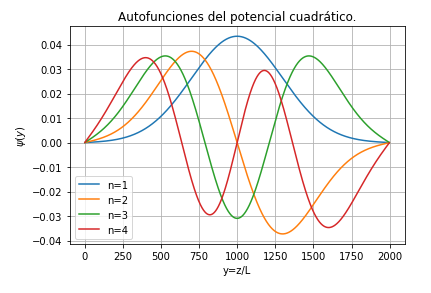
\includegraphics[scale=0.5]{sqr_eigf.png}
\caption{Autofunciones del potencial cuadrático en la variable adimensional $y=x/L$}
    \label{fig:my_label}
\end{figure}

Y los autovalores asociados a dichas autofunciones:

\begin{figure}[htp]
    \centering
    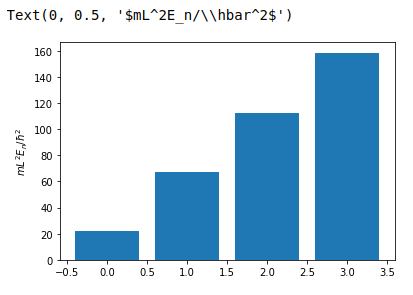
\includegraphics[scale=0.5]{sqr_eigv.png}
    \caption{Autovalores del potencial cuadrático en unidades $mL^2E_n/\hbar^2$}
    \label{fig:my_label}
\end{figure}

\newpage
Obteniendo el módulo cuadrado de las autofunciones, las densidades de probabilidad son

\begin{figure}[h]
    \centering
    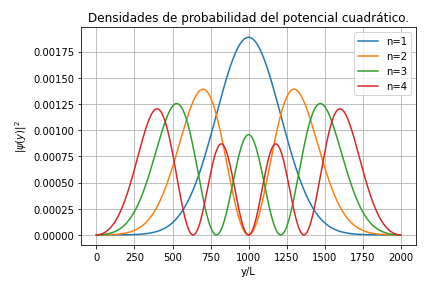
\includegraphics[scale=0.45]{sqr_dens.png}
    \caption{Autovalores del potencial cuadrático en unidades $mL^2E_n/\hbar^2$}
    \label{fig:my_label}
\end{figure}

\end{document}
